\documentclass[11pt]{article}
\usepackage{fullpage}
\usepackage{amsmath}    % need for subequations
%\usepackage{graphicx}   % need for figures
\usepackage{verbatim}   % useful for program listings
\usepackage{color}      % use if color is used in text
\usepackage{subfigure}  % use for side-by-side figures
\usepackage{hyperref}   % use for hypertext links, including those to external documents and URLs
\usepackage[pdftex]{graphicx}


\title{CMSC 12300 Final Project}
\author{Andy Liu and Nelson Auner}
\begin{document}
\maketitle
\section{Introduction}

%%Maybe move this subsection out of the introduction
\subsection{Logistic regression of census data}
Our project investigates predicting whether a household self reports that its income is over or under \$50,000, based on census data. 
We aim to find the best classification method within the subset of logistic regression classifiers. Logistic regression transforms the predictors to
\begin{equation}
\pi(X) = \frac{e^{(X\beta)}}{1+e^{(X\beta)}}
\end{equation}
this projects the space of $X \beta$ to the interval $[0,1]$, allowing us to view the result as the probability that our outcome is 1. Although more complicated than a basic regression mode $Y = X\beta$, logistic regression allows us to predict a binary outcome, while resulting in more interpretable coefficients $\beta$ than black box methods such as neural networks or random forest. 
\subsection{Goals and summary of results}
Our main goals, put succintly, were to find and compare the best prediction method by testing various combination of predictors. For each prediction method, we wanted to quantify the effectiveness of that algorithm. Given the large proportion of observations with missing values, we also wanted to examine the effects of filling in missing observations with values. 

\section{Description of the Data set}
Our analysis is on the Census-Income (KDD) Data Set, a classic machine learning dataset as well as applicable machine 
The census data we used is made freely available from
\href{http://archive.ics.uci.edu/ml/datasets/Census-Income+%28KDD%29}{the UC-Irvine Machine Learning Repository} 
The most pertinant characteristic of the data set is that the "over 50K" variable only takes on a value of true for 6.2% of the observations. As we noted in our original proposal, this means that a majority classifiers--predicting that income is under 50K for all observations, would have been "93.8% accurate". However, this is not a useful predictor, since we do not know if a set of new observations would be reprentative at all of our current data. In addition, it's important to consider weighting the relative importance of assigning a false positive vs. a false negative: for a business/marketing application of the data, it may be more important to predict all of the observations with income > \$50K, than correctly predict observation under \$50K. In this sense, the majority classifier is undesireable, asit predicts no observations with income > \$50K, regardless of information.

\section{Initial analysis}
Our inital analysis was done in R, and much work was required to find and adapt the necessary statistical methods for use in python. 
We used the Akaike Information Criteria (AIC), defined as $AIC = 2k - 2ln(L)$, where $k$ is the number of the parameters in the model, and $L$ is the maximized value of the likelihood function - in our case, the logistical regression equation defined above. By maximizing AIC, we produced a subset of predictors that AIC evaluated as the "best" predictor sets. We noticed that among single-variable predictive methods, the education variable was one of the most effective, with a false positive error rate of 5% false negative error rate of .7%. However, these rates are not accurate measures of performance, because we are testing our predictor with the same data we used to train. 

\section{Cross Validation}
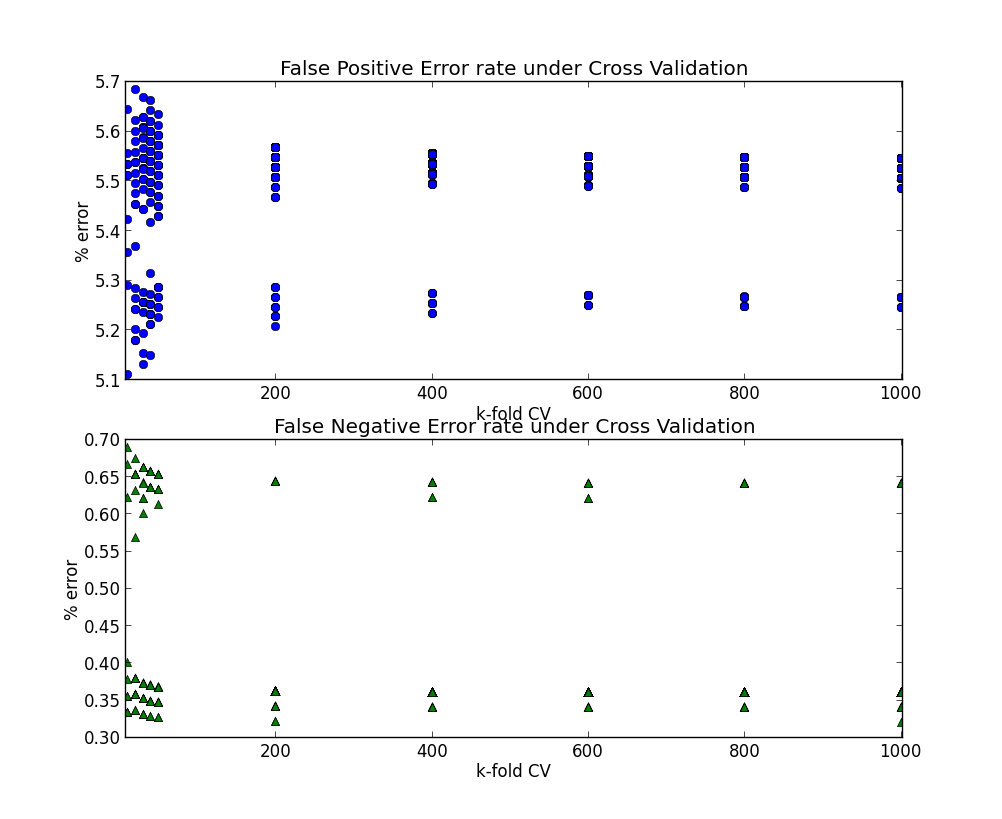
\includegraphics[width = 20cm]{CV_5K_1Kfold.png}
\end{document}
